\section{Economic Interpretation}
\label{sec:economic}

The NED framework represents each article through two quantities: an
impact magnitude $s_k$ and a decay rate $\lambda_k$. These parameters
provide a way to examine which kinds of text the model associates with
large and persistent adjustments to a volatility forecast. Their
interpretation is conditional on the residual loading $a$, the intercept
$b$, and the clipping operation in Equation~\eqref{eq:residual}.
In particular, $s_k$ is an internal signal magnitude; the initial
contribution to the unclipped log-variance correction is $a s_k$.
The parameters describe predictive associations rather than causal
responses to externally identified news shocks.

We organize the analysis around three questions: how long does news move
volatility (Section~\ref{sec:timescale}), how does news content shape the
impact (Section~\ref{sec:categories}), and what dimension of the text
representation does the model use (Section~\ref{sec:sentiment})?
The analysis uses the BTC 4-hour model and the 7,845 retained articles
that enter at least one of its out-of-sample forecasts across the six
expanding windows. Each article contributes one parameter pair estimated
by the corresponding window's fitted model.

\subsection{Timescale: How long does news move volatility?}
\label{sec:timescale}

\begin{figure}[htbp]
\centering
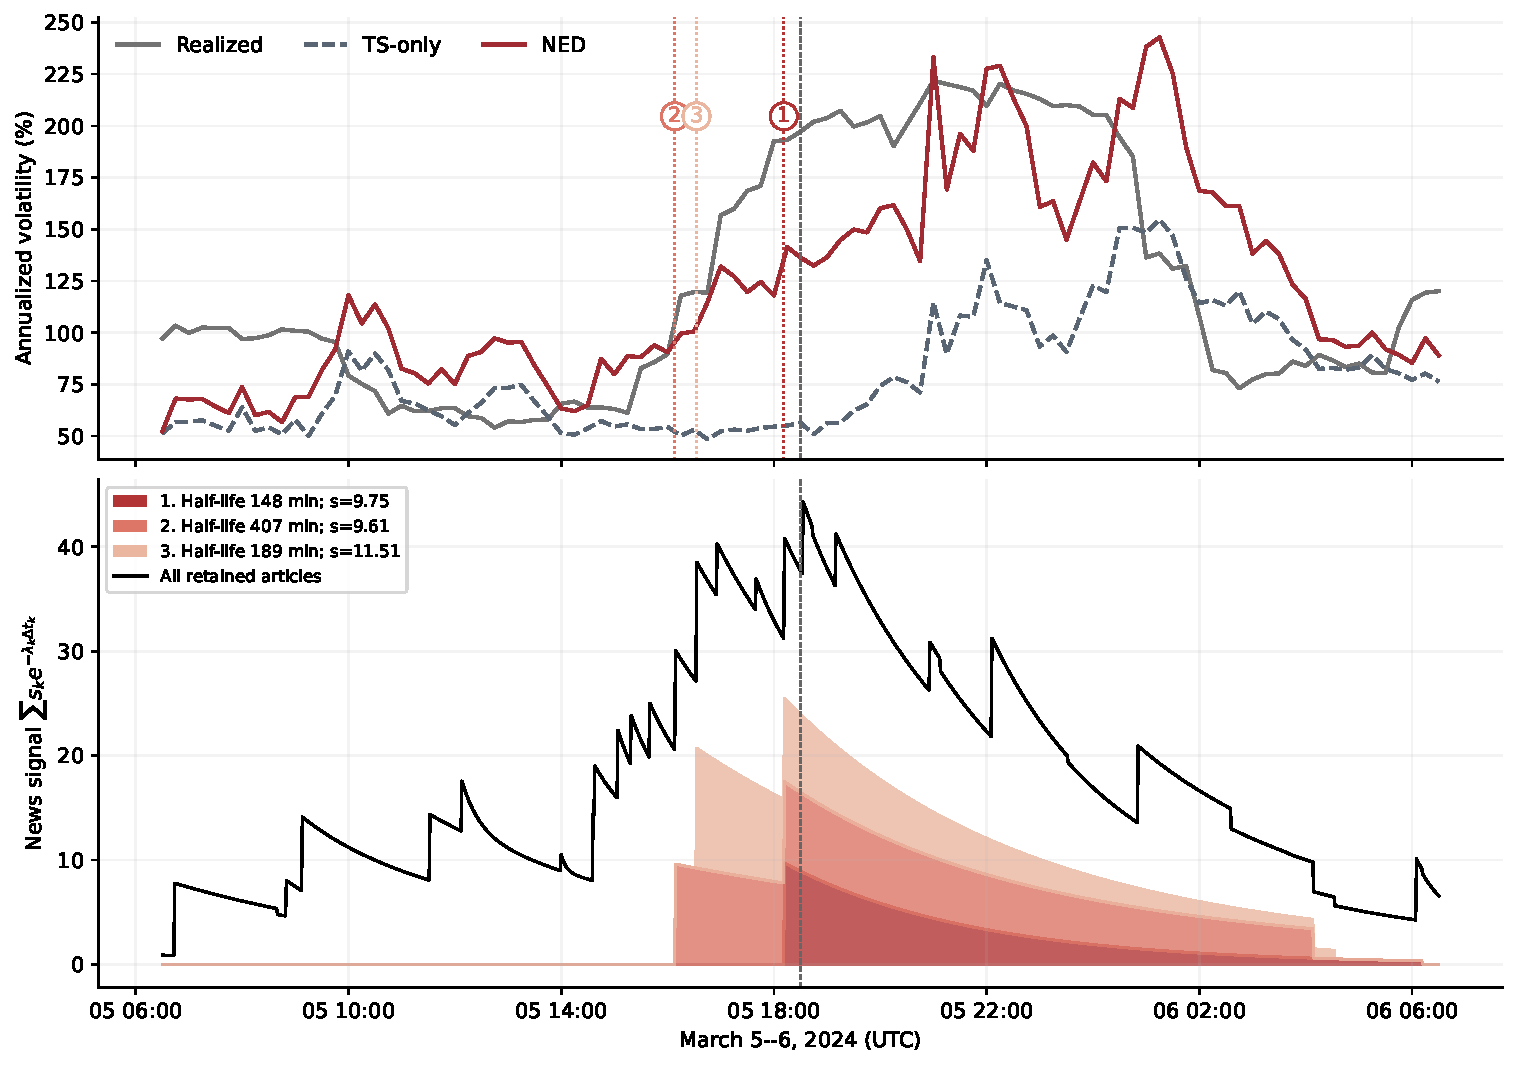
\includegraphics[width=\textwidth]{figures/casestudy.pdf}
\caption{News-driven forecast adjustment around 5 March 2024. The upper
panel compares 4-hour annualized realized volatility with TS-only and NED
forecasts. The numbered vertical markers identify the three articles
with the largest remaining signals at 18:30 UTC. The lower panel stacks
their learned signals, $s_k\exp(-\lambda_k\Delta t_k)$, and overlays the
sum for all retained articles in the twelve-hour lookback. The dashed
vertical line marks the selection time. The signals are inputs to the
residual map, rather than additive contributions to annualized volatility.}
\label{fig:casestudy}
\end{figure}

Figure~\ref{fig:casestudy} examines the same forecasting episode around
Bitcoin's March 2024 record high. To select the displayed articles
systematically, we fix the forecast timestamp at 5 March, 18:30 UTC,
and rank eligible articles by their remaining signal
$s_k\exp(-\lambda_k\Delta t_k)$. Table~\ref{tab:case_articles} reports
the three highest-ranked articles. They discuss the record price, its
possible implications, and the subsequent decline. The corresponding
half-lives are approximately 148, 407, and 189 minutes. The
forward-looking article therefore receives the most persistent response,
while the decline report has the largest initial magnitude.

\begin{table}[htbp]
\centering\small
\caption{Articles highlighted in the forecasting episode}
\label{tab:case_articles}
\begin{adjustbox}{max width=\textwidth}
\begin{tabular}{cp{9cm}rr}
\toprule
No. & Article & $s$ & $h_{1/2}$ (min) \\
\midrule
1 & Bitcoin Soars to a Record -- but What's the Price? And What Was the Old All-Time High? & 9.75 & 147.6 \\
2 & Bitcoin Hit a Record High. Here's What Might Happen Next & 9.61 & 407.1 \\
3 & Bitcoin Tumbles 10\% After Hitting Record High; Triggers \$1B Crypto Liquidations & 11.51 & 188.6 \\
\bottomrule
\end{tabular}

\end{adjustbox}
\tabnote{Articles are ordered by remaining signal at 5 March 2024,
18:30 UTC. Magnitudes and half-lives are extracted from the third
expanding-window BTC 4-hour model.}
\end{table}

The news signals contribute to a separation between the NED and TS-only
forecasts during the episode. The residual loading is positive
($a=0.0468$), so a larger aggregate signal raises the variance forecast
until the correction reaches its cap. The figure also makes clear why
the analysis should not be read as a causal event study: a report of an
ongoing price decline survives the deterministic recap filter, and
realized variance is measured over an overlapping forward horizon.
The episode illustrates the model's mechanism and the differences among
article persistence estimates, rather than identifying an exogenous
effect of any one publication.

\begin{figure}[htbp]
\centering
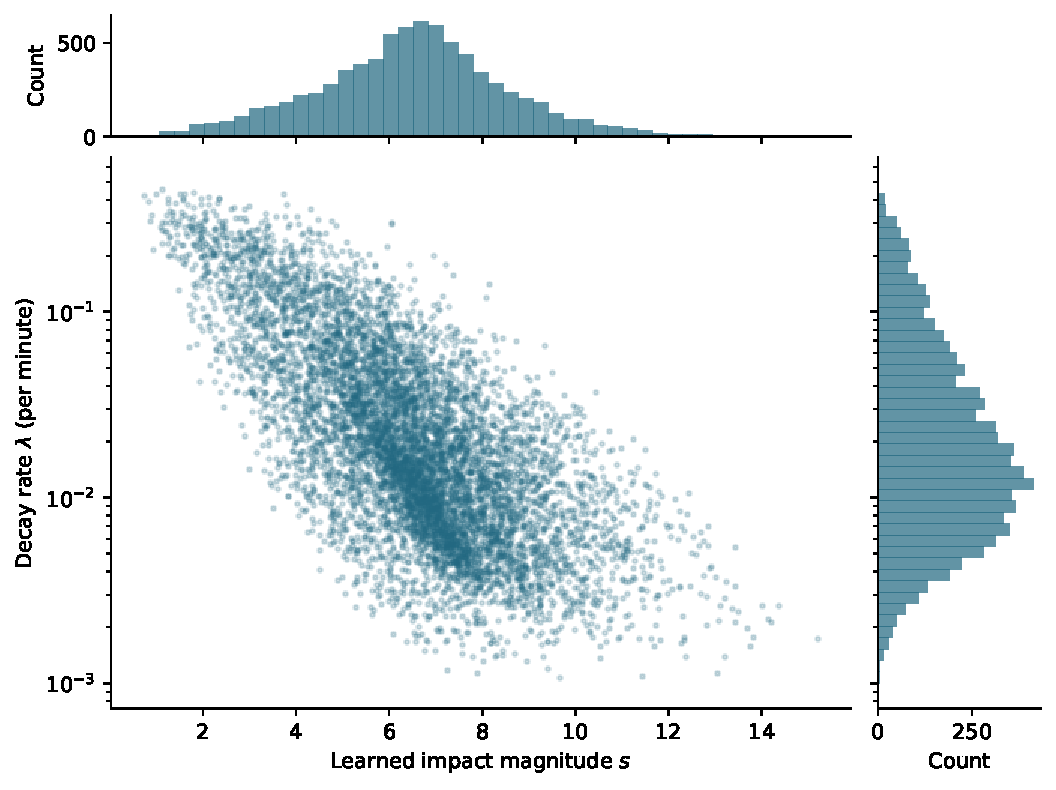
\includegraphics[width=0.85\textwidth]{figures/distribution.pdf}
\caption{Joint distribution of learned article magnitude $s$ and decay
rate $\lambda$ in the BTC 4-hour models. Each point is one of 7,845
articles entering an out-of-sample forecast; the marginal distributions
appear above and to the right. Decay rates are measured per minute and
shown on a logarithmic axis. Larger magnitudes tend to be associated with
slower decay.}
\label{fig:joint}
\end{figure}

Figure~\ref{fig:joint} examines whether heterogeneous persistence also
appears across the full test sample. The mean learned magnitude is 6.50
and its median is 6.55. The median half-life is 42.7 minutes, with an
interquartile range from 16.8 to 88.8 minutes. Only 3.4\% of articles
have half-lives exceeding four hours. The model thus assigns most
retained news a relatively short period of relevance, while allowing a
smaller group to influence forecasts for several hours.

Magnitude and decay rate exhibit a negative rank association
(Spearman's $\rho=-0.687$). Articles with larger internal signals tend to
retain those signals longer. This relationship is not imposed by an
explicit constraint linking the two output coordinates, although both
are produced by the same news head and optimized under the same loss.
Pooling parameters across independently fitted windows also introduces
variation in their scale. The association is therefore a descriptive
property of the fitted news branch, rather than evidence that large
economic shocks must necessarily dissipate more slowly.

\subsection{News category and impact heterogeneity}
\label{sec:categories}

To examine whether the learned parameters vary across economically
meaningful information types, we assign the retained test-sample
articles to twelve mutually exclusive news categories. The category
labels are constructed after reactive filtering and are used only for
interpretation. They are not inputs to the volatility model and do not
affect its training or forecast evaluation.

Classification proceeds in two stages. First, deterministic title
patterns identify recurring branded columns and newsletters and assign
them to Newsletter Series. Second, the remaining articles are classified
with the zero-shot natural language inference model
\texttt{MoritzLaurer/\allowbreak ModernBERT-large-zeroshot-v2.0}.\footnote{Model and
configuration: \url{https://huggingface.co/MoritzLaurer/ModernBERT-large-zeroshot-v2.0}.
We fix checkpoint revision
\texttt{a51e07b524299e309dd2b88d48b0cfa2bd9ec598}.}
Its candidate labels are Macro, Geopolitical, Regulatory and Legal,
Security and Crime, Institutional Flows, Protocol and Infrastructure,
On-Chain Flows, Product Adoption, Market Commentary, Opinion and
Editorial, and Other. Each label is accompanied by a short definition
in a hypothesis about the event reported by the article. We apply
softmax across the eleven entailment scores, assign the highest-scoring
label, and use Other when that score is below 0.25. Article premises are
truncated to fit the 512-token input limit.

\begin{table}[htbp]
\centering\small
\caption{News category and learned impact heterogeneity (BTC, 4-hour)}
\label{tab:news-taxonomy}
\begin{adjustbox}{max width=\textwidth}
\begin{tabular}{lrrrrr}
\toprule
Category & $N$ & Mean $s$ & Std.\ $s$ & Median $h_{1/2}$ (min) & Mean $as$ \\
\midrule
Macro & 450 & 8.96 & 2.22 & 78.1 & 0.288 \\
Geopolitical & 134 & 8.08 & 2.17 & 47.1 & 0.245 \\
Newsletter series & 712 & 6.85 & 2.23 & 34.4 & 0.223 \\
On-chain flows & 399 & 6.73 & 1.94 & 51.1 & 0.206 \\
Institutional Flows & 849 & 6.62 & 1.91 & 37.0 & 0.218 \\
Other & 663 & 6.44 & 1.92 & 41.3 & 0.207 \\
Market Commentary & 2287 & 6.43 & 1.91 & 43.0 & 0.205 \\
Regulatory/Legal & 816 & 6.04 & 1.58 & 45.4 & 0.209 \\
Security/Crime & 165 & 5.81 & 1.61 & 52.1 & 0.185 \\
Protocol/Infrastructure & 436 & 5.79 & 1.85 & 56.0 & 0.180 \\
Product Adoption & 379 & 5.74 & 1.54 & 43.2 & 0.170 \\
Opinion/Editorial & 555 & 5.63 & 1.64 & 25.0 & 0.181 \\
\bottomrule
\end{tabular}

\end{adjustbox}
\tabnote{Each of the 7,845 articles receives equal weight. Categories are
ordered by mean $s$. The final column incorporates the residual loading
from the article's expanding window and reports the mean initial
unclipped log-variance contribution $a s$. Half-lives are measured in
minutes. Labels are automatically generated descriptive annotations.}
\end{table}

Table~\ref{tab:news-taxonomy} shows substantial variation across event
types. Macro news has the largest mean magnitude, 8.96, and the longest
median half-life, 78.1 minutes. Geopolitical news ranks second in
magnitude at 8.08, but its median half-life is 47.1 minutes. Both groups
also rank highest when magnitudes are multiplied by their fitted
window-specific residual loadings. The model therefore associates
broad macroeconomic information with a particularly large and persistent
forecast adjustment, while the distinction for geopolitical articles
is clearer in magnitude than in duration.

The remaining categories illustrate why magnitude and persistence
should be examined separately. Newsletter Series has a relatively
large mean magnitude of 6.85 but a shorter median half-life of
34.4 minutes. Protocol/Infrastructure and Security/Crime have lower
mean magnitudes, 5.79 and 5.81, yet median half-lives of 56.0 and
52.1 minutes. Opinion/Editorial has the lowest mean magnitude, 5.63,
and the shortest median half-life, 25.0 minutes. Product Adoption
also receives a relatively small magnitude, 5.74, although its
43.2-minute median half-life is close to the sample-wide value.
The temporal ordering is thus not a simple restatement of the
magnitude ordering.

These comparisons concern article-level fitted parameters and should
be distinguished from the volume of coverage. Market Commentary is
the largest category, with 2,287 articles, whereas Macro and
Geopolitical contain 450 and 134. Category composition can differ
across the independently fitted windows, and the labels themselves
are automated annotations: 613 articles fall below the confidence
threshold and are assigned to Other. The results provide an
economically recognizable description of the learned news signals,
while leaving causal explanations of category differences open.


\subsection{Sentiment versus event content: What does CryptoBERT contribute?}
\label{sec:sentiment}

An article representation can encode both the direction of a statement
and the nature of the event it describes. To examine their relationship
to the learned news parameters, we use the precomputed three-class
probabilities from \texttt{ProsusAI/finbert} \citep{Araci2019}.
These sentiment scores are distinct from the CryptoBERT embeddings
used by the main forecasting model. For each article, an individual
class is decisive when its probability exceeds 0.60; otherwise the
article is assigned to the ambiguous group.

\begin{table}[htbp]
\centering\small
\caption{FinBERT sentiment and learned article magnitude (BTC, 4-hour)}
\label{tab:sentiment-vs-s-finbert}
\begin{adjustbox}{max width=\textwidth}
\begin{tabular}{lrrrrr}
\toprule
Group & $N$ & Mean $s$ & Median $s$ & Std.\ $s$ & Median $h_{1/2}$ (min) \\
\midrule
Positive-decisive & 1841 & 6.941 & 7.015 & 2.036 & 46.9 \\
Neutral-decisive & 2736 & 5.580 & 5.864 & 1.595 & 33.4 \\
Negative-decisive & 2315 & 7.286 & 7.269 & 2.127 & 52.8 \\
Ambiguous & 953 & 6.382 & 6.538 & 1.829 & 44.7 \\
\bottomrule
\end{tabular}

\end{adjustbox}
\tabnote{A decisive class has probability greater than 0.60. All other
articles are ambiguous. Probabilities are matched to articles using
their original asset-specific row indices and verified publication
timestamps. Each article receives equal weight.}
\end{table}

Table~\ref{tab:sentiment-vs-s-finbert} shows that negative-decisive
articles have a mean magnitude of 7.29, compared with 6.94 for
positive-decisive articles and 5.58 for neutral-decisive articles.
Their median half-life is also longer: 52.8 minutes for negative,
46.9 minutes for positive, and 33.4 minutes for neutral articles.
A two-sided Mann--Whitney comparison between negative and positive
magnitudes yields $p=1.86\times10^{-7}$. The difference remains
significant at decisiveness thresholds of 0.50 and 0.70. These
comparisons indicate a polarity-related asymmetry in the fitted
parameters, but do not identify the leverage mechanism of an
asset-pricing model.

Ambiguous articles have a mean magnitude of 6.38 and a median half-life
of 44.7 minutes. Their magnitude distribution does not differ
significantly from the combined decisive group at the 0.60 cutoff
($p=0.130$). Moreover, this comparison changes with the decisiveness
threshold. The evidence therefore supports a negative--positive
difference more clearly than a general claim that ambiguity itself
induces a distinct volatility response.

The sentiment comparison describes how the full model organizes its
article signals; it does not determine whether sentiment alone would
be sufficient for forecasting. Section~\ref{sec:news_representations}
addresses that separate question by replacing the article
representation and refitting the news branch under matched conditions.
